\documentclass[border=15pt, multi, tikz]{standalone}

\usepackage{tikz}
\usetikzlibrary{quotes,arrows.meta}
\usetikzlibrary{positioning}
\def\edgecolor{rgb:blue,4;red,1;green,4;black,3}
\newcommand{\midarrow}{\tikz \draw[-Stealth,line width =0.8mm,draw=\edgecolor] (-0.3,0) -- ++(0.3,0);}
\usepackage{Box}
\usepackage{RightBandedBox}

\def\ConvColor{rgb:blue,5;green,2.5;white,5}
\def\ConvReluColor{rgb:blue,5;green,5;white,5}
\def\PoolColor{rgb:red,1;black,0.3}
\def\DcnvColor{rgb:blue,5;green,2.5;white,5}
\def\UnpoolColor{rgb:yellow,5;red,2.5;white,5}
\def\SoftmaxColor{rgb:magenta,5;black,7}

\usetikzlibrary{3d} %for including external image 

\begin{document}

\begin{tikzpicture}
\tikzstyle{connection}=[ultra thick,every node/.style={sloped,allow upside down},draw=\edgecolor,opacity=0.7]
%%%%%%%%%%%%%%%%%%%%%%%%%%%%%%%%%%%%%%%%%%%%%%%%%%%%%%%%%%%%%%%%%%%%%%%%%%%%%%%%%%%%%%%%
%% Draw Layer Blocks
%%%%%%%%%%%%%%%%%%%%%%%%%%%%%%%%%%%%%%%%%%%%%%%%%%%%%%%%%%%%%%%%%%%%%%%%%%%%%%%%%%%%%%%%
%%%%%%%%%%   

\node[canvas is zy plane at x=0]  (mask1) at (0,0,0)   {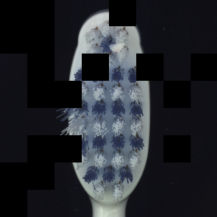
\includegraphics[width=12cm,height=12cm]{img/sub-img/toothbrush-defective-masked1.png}};
\node[canvas is zy plane at x=3]  (mask2) at (2,3,0)   {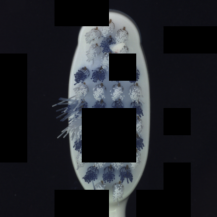
\includegraphics[width=12cm,height=12cm]{img/sub-img/toothbrush-defective-masked2.png}};
\node[canvas is zy plane at x=6]  (mask3) at (4,6,0)   {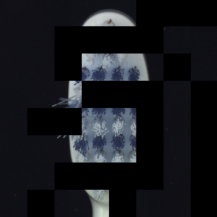
\includegraphics[width=12cm,height=12cm]{img/sub-img/toothbrush-defective-masked3.png}};

% CONVOLUTION
\pic[shift={(20,0,0)}] at (mask1) {RightBandedBox={name=c1,caption=CONVOLUTION,
        fill=\ConvColor,bandfill=\ConvReluColor,
        height=40,width={2,2,2,2,2},depth=40}};

% CONVOLUTION
\pic[shift={(3,0,0)}] at (c1-east) {RightBandedBox={name=c2,caption=CONVOLUTION,
        fill=\ConvColor,bandfill=\ConvReluColor,
        height=40,width={2,2,2,2,2},depth=40}};

% CONVOLUTION
\pic[shift={(3,0,0)}] at (c2-east) {RightBandedBox={name=c3,caption=CONVOLUTION,
        fill=\ConvColor,bandfill=\ConvReluColor,
        height=40,width={2,2,2,2,2},depth=40}};

% CONVOLUTION
\pic[shift={(3,0,0)}] at (c3-east) {RightBandedBox={name=c4,caption=CONVOLUTION,
        fill=\ConvColor,bandfill=\ConvReluColor,
        height=40,width={2,2,2,2,2},depth=40}};


\node[canvas is zy plane at x=0]  (pred1) at (50,0,0)  {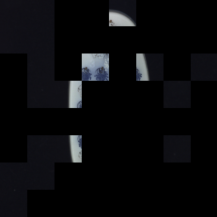
\includegraphics[width=12cm,height=12cm]{img/sub-img/toothbrush-extracted1.png}};
\node[canvas is zy plane at x=3]  (pred2) at (52,3,0)  {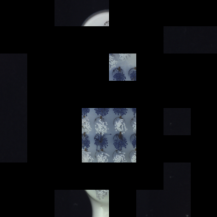
\includegraphics[width=12cm,height=12cm]{img/sub-img/toothbrush-extracted2.png}};
\node[canvas is zy plane at x=6]  (pred3) at (54,6,0)  {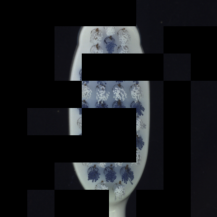
\includegraphics[width=12cm,height=12cm]{img/sub-img/toothbrush-extracted3.png}};

\draw [connection]  (mask1.center)   -- node {\midarrow} (c1-west);
\draw[->, densely dashed]
(mask1.north east) -- (c1-nearnorthwest)
(mask1.south east) -- (c1-nearsouthwest)
(mask1.south west)  -- (c1-farsouthwest)
(mask1.north west)  -- (c1-farnorthwest)
;

\draw [connection]  (c1-east)   -- node {\midarrow} (c2-west);
\draw[->, densely dashed]
(c1-nearnortheast) -- (c2-nearnorthwest)
(c1-nearsoutheast) -- (c2-nearsouthwest)
(c1-farsoutheast)  -- (c2-farsouthwest)
(c1-farnortheast)  -- (c2-farnorthwest)
;
\draw [connection]  (c2-east)   -- node {\midarrow} (c3-west);
\draw[->, densely dashed]
(c2-nearnortheast) -- (c3-nearnorthwest)
(c2-nearsoutheast) -- (c3-nearsouthwest)
(c2-farsoutheast)  -- (c3-farsouthwest)
(c2-farnortheast)  -- (c3-farnorthwest)
;
\draw [connection]  (c3-east)   -- node {\midarrow} (c4-west);
\draw[->, densely dashed]
(c3-nearnortheast) -- (c4-nearnorthwest)
(c3-nearsoutheast) -- (c4-nearsouthwest)
(c3-farsoutheast)  -- (c4-farsouthwest)
(c3-farnortheast)  -- (c4-farnorthwest)
;


\draw [connection]   (c4-east)  -- node {\midarrow} (pred1.center);
\draw[->, densely dashed]
(c4-nearnortheast) -- (pred1.north east) 
(c4-nearsoutheast) -- (pred1.south east) 
(c4-farsoutheast)  -- (pred1.south west)
(c4-farnortheast)  -- (pred1.north west)
;
\node[canvas is zy plane at x=0]  (pred1) at (50,0,0)  {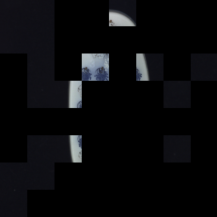
\includegraphics[width=12cm,height=12cm]{img/sub-img/toothbrush-extracted1.png}};


\end{tikzpicture}
\end{document}\grid
